% Content for the test report for LSP-00-10

\subsection{API Aspect tests}

This test case exercises the LSP via the API Aspect only.

It verifies the ability to perform a variety of basic table scan queries.

Data for the test are primarily taken from the Object-like AllWISE (coadded) Source Catalog,
and the ForcedSource-like Multi-Epoch Photometry table,
except as noted below.

\subsubsection{Step 2}

The tests were performed primarily from an Apple Macbook Air computer running OS X 10.11.6,
connected to the Internet wirelessly at IPAC and other locations.
Queries requiring larger downloads were performed on an Apple iMac computing running OS X 10.11.6,
connected to the IPAC wired institutional network.

The tests were performed using Jupyter 5.4.1 on Python 3.6.1, and the notebook was accessed using version 11.1 of the Safari browser.

\subsubsection{Step 3}

A connection was established to the PDAC network environment using the NCSA VPN at \texttt{vpn.ncsa.illinois.edu}.

The \verb|dbserv| version 0 pseudo-TAP service was accessed at:

\begin{center}
\texttt{http://lsst-qserv-dax01.ncsa.illinois.edu:5000/db/v0/tap/sync}
\end{center}

\subsubsection{Step 4 --- Very small queries}

A target object was chosen near ( ra=4, dec=0 ):
\verb|source_id| ``\verb|0045p000_ac51-034420|'', \verb|cntr| 45100001351034420, \verb|ra| 3.9967364, \verb|decl| 0.002037.

Since the \verb|cntr| attribute is not indexed, a search for a row matching this unique ID in the Object-like database,
or a search for rows matching this as the parent-object ID in the ForcedSource-like database,
will result in a table scan.
If combined with a spatial restriction, this table scan can be limited to a subset of the database shards maintained by Qserv.

Following the guidance in LDM-540,
although these queries scan up to the full number of rows in these two tables (758 million and 42 billion, respectively),
they return only a small amount of data in the end.

A series of increasing-diameter cone searches were done,
using the special Qserv spatial-restriction function \verb|qserv_areaspec_circle|,
to trace out the behavior of Qserv as the fraction of shards scanned increased.

The query texts were:
\texttt{SELECT cntr, ra, decl, w1mpro, w2mpro FROM wise\_00.allwise\_p3as\_psd WHERE qserv\_areaspec\_circle(3.9967364,0.002037,} $r$ \texttt{) AND cntr=45100001351034420} for the Object-like table, and
\texttt{SELECT cntr, cntr\_mf, ra, decl, mjd, w1mpro\_ep, w2mpro\_ep FROM wise\_00.allwise\_p3as\_mep WHERE qserv\_areaspec\_circle(3.9967364,0.002037,} $r$ \texttt{) AND cntr\_mf=45100001351034420} for the ForcedSource-like table,
where the radius $r$ is in degrees.

The queries were carried out for radii in powers of two from $1/1024$ through $64$, and for the half-sky radius $89.9$.
Finally, an all-sky version was carried out by omitting the \verb|qserv_areaspec_circle| function.

All the queries returned the same results: a single row in the case of the Object-like queries,
and 24 rows of forced photometry associated with that object for the ForcedSource-like queries.
Successfully completing the half-sky and all-sky ForcedSource queries via \verb|dbserv| required raising the \verb|webserv|
timeout from 30 minutes to two hours.

\begin{table}[h]
\centering
\begin{tabular}{r r r r}
Radius (deg.) & Sky Area (sq. deg.) & Object elapsed time (s) & ForcedSource elapsed time (s) \\ \hline
0.0010 & $3.00\times 10^{-6}$ & 0.54 & 0.83 \\
0.0020 & $1.20\times 10^{-5}$ & 0.22 & 0.33 \\
0.0039 & $4.79\times 10^{-5}$ & 0.22 & 0.35 \\
0.0078 & $1.92\times 10^{-4}$ & 0.22 & 0.37 \\
0.0156 & $7.67\times 10^{-4}$ & 0.21 & 0.40 \\
0.0313 & $3.07\times 10^{-3}$ & 0.22 & 0.41 \\
0.0625 & $1.23\times 10^{-2}$ & 0.21 & 1.03 \\
0.125 & $4.91\times 10^{-2}$ & 0.21 & 0.67 \\
0.25 & $1.96\times 10^{-1}$ & 0.22 & 0.46 \\
0.5 & $7.85\times 10^{-1}$ & 0.23 & 0.40 \\
1.0 & $3.14\times 10^{0}$ & 0.33 & 0.45 \\
2.0 & $1.26\times 10^{1}$ & 0.92 & 0.62 \\
4.0 & $5.02\times 10^{1}$ & 1.84 & 3.55 \\
8.0 & $2.01\times 10^{2}$ & 5.22 & 5.79 \\
16.0 & $7.99\times 10^{2}$ & 16.59 & 17.27 \\
32.0 & $3.13\times 10^{3}$ & 55.67 & 59.13 \\
64.0 & $1.16\times 10^{4}$ & 207.62 & 942.73 \\
89.9 & $2.06\times 10^{4}$ & 380.07 & 2365.89 \\
all-sky & $4.13\times 10^{4}$ & 929.33 & 4506.66
\end{tabular}
\caption{Table-scan results for small queries on Object- and ForcedSource-like tables}
\label{tab:lsp-00-10-simple-scan-timings}
\end{table}

\begin{figure}
  \centering
  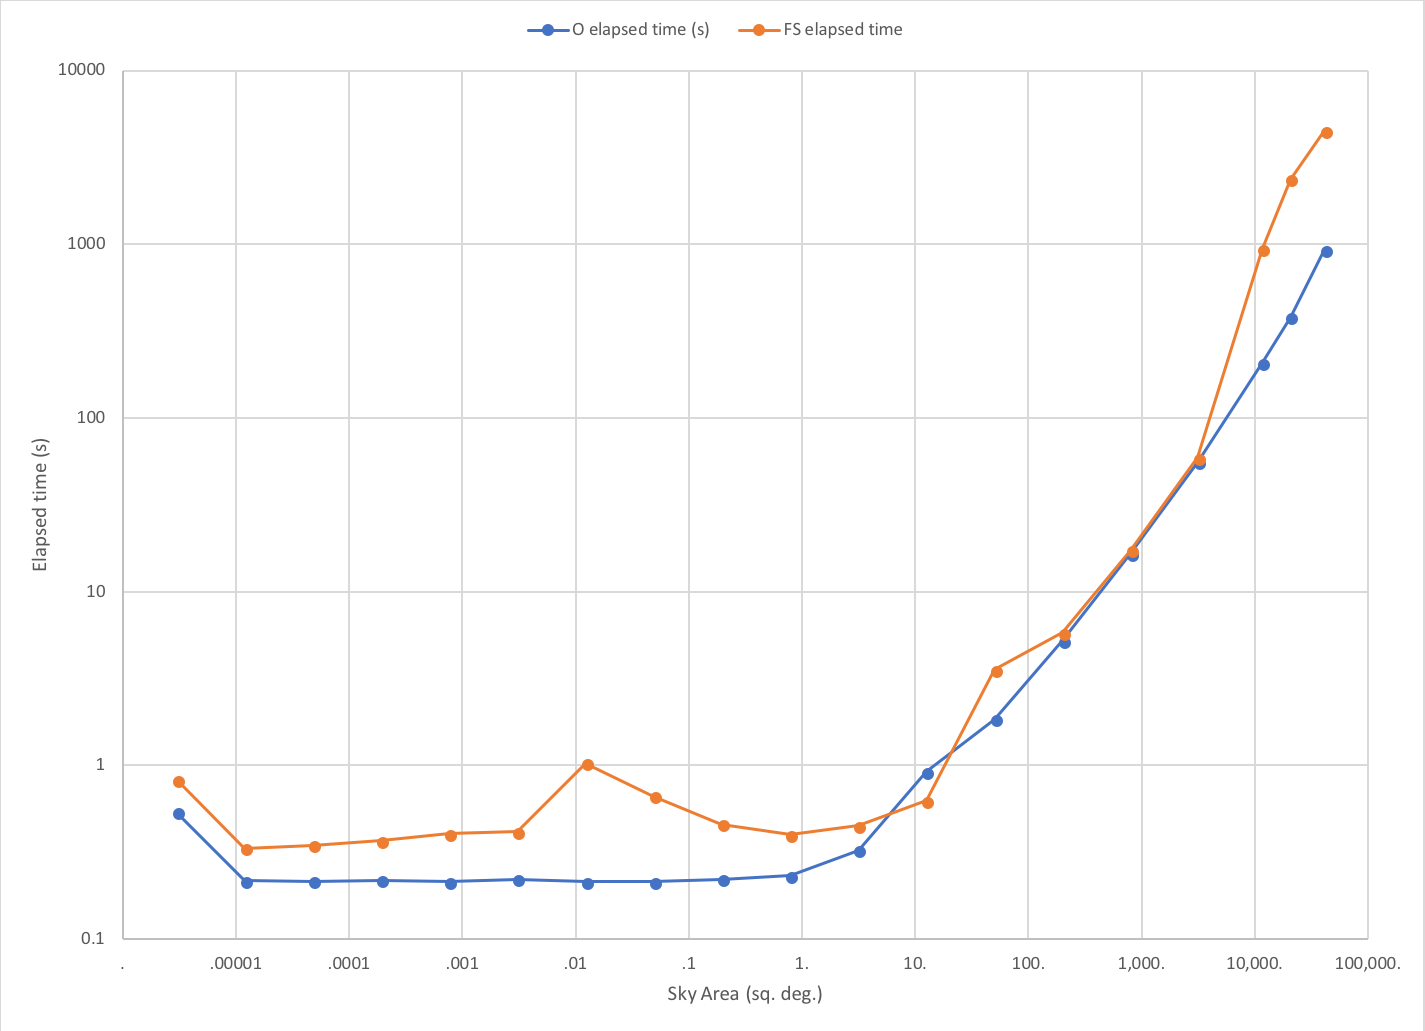
\includegraphics[width=4in]{lsp-00-10/SimpleScans.png}
  \caption{Query results for the Object-like AllWISE Source Catalog}
  \label{fig:lsp-00-10-simple-scan-plot}
\end{figure}

\subsubsection{Step 4 --- Low volume queries}

The ``low volume'' query specification is for queries which are intended to complete within an interactive-work-friendly time of 10 seconds.
These were intended to be limited in scope to a fraction of the Object database limited to no more than 10 million rows.
In the logic of Qserv this has to be a spatial restriction, in order to permit the number of shards searched to be reduced.
As a fraction of the eventually expected Object database, this is approximately 1/2,000.
If this is expressed spatially, for the LSST survey it would be approximately 10 square degrees,
or the size of a single focal plane field.
This is also approximately the size expected for coadd ``patches''.
Accordingly, in these tests we explored query sizes of approximately this spatial area, as well as of approximately the same number of rows:

\begin{itemize}
\item{a 2-degree-radius cone search around the reference Object above, with area 12.6 square degrees,
and including 170,503 rows; and}
\item{a 16-degree-radius cone search around the reference Object above, with area 799 square degrees,
and including 10,546,932 rows.}
\end{itemize}

Note that for the latter query spatial-restriction ``denominator'' even the one-row identifier query above does currently take more than the specified 10 seconds (16.6s --- see above);
however, there was no expectation that the final Qserv performance would have been met by the current deployment.

For reference, as a fraction of the AllWISE Object-like database, the 1/2,000 ratio above corresponds to 379,000 rows, in between the two spatial-restriction choices explored.

The expected size of the result set supported for such a query is specified as 0.1 GB.
Scaled by the ratio of the number of rows in the WISE dataset (758M) to the expected Object database size of approximately 20G rows, this would be about 4 MB.
Nevertheless, queries approaching 100MB in result set size were performed.

To exercise the space, two types of queries were run, one returning a minimal set of columns (\texttt{cntr, ra, decl, w1mpro, w2mpro, w3mpro, w4mpro}) and the other returning all columns (\texttt{SELECT *}).
For each spatial region and each query type, a series of queries was run with different restrictions on the value of \verb|w1mpro| (which was not indexed) to scan the space of result set sizes.

The queries in this section were carried out via the \verb|curl| command, executed from within a test notebook,
because this permitted separately measuring the query execution time in the DAX service and the data transfer time from DAX to the client host.
(The \verb|curl| command has an option for reporting the elapsed time until data begins to be returned from the request.)
The notebook was running on the \texttt{lsst-lspdev.ncsa.illinois.edu/nb} JupyterLab service.
The file transfer times recorded for the largest downloads (in the high 10s of MB) corresponded to intra-NCSA delivered bandwidths from the \verb|dbserv| service to the Jupyter Notebook processes of 200-300 MB/s.
It was not part of this test specification to perform tests of multiple simultaneous downloads.

Note that the performance of these queries was measured on an otherwise unloaded system.
With the current Qserv configuration, all of these are believed to have been carried out as ``shared scans'',
which could have been joined with any other pending shared scans and potentially taken much longer.
The currently configured threshold for performing a shared scan,
as opposed to immediate execution, is a query area larger than about 3 square degrees.
On an unloaded system it is difficult to see any difference in performance,
and there is no explicit feedback available from Qserv as to which mode of execution is being used for a particular query.
The shared-scan-threshold configuration parameter can be revisited as operational experience is gained.

Approximately one in twenty of the queries performed failed randomly on the first attempt,
but succeeded when immediately repeated.
This is believed to be due to an issue in the communication protocol between \verb|dbserv| and Qserv,
rather than a problem in Qserv itself.
There was no correlation with query size.

\begin{table}[h]
\centering
\begin{tabular}{r r r r r r r r}
 & & \multicolumn{3}{c}{Narrow column selection} & \multicolumn{3}{c}{\texttt{SELECT *}} \\ \hline
\texttt{w1mpro} &  & query & transfer &  & query & transfer &  \\
cut & rows & time (s) & time (s) & bytes & time(s) & time (s) & bytes \\ \hline
5 & 9 & 0.463 & 0.002 & 984 & 0.501 & 0.002 & 31,945 \\
6 & 15 & 0.420 & 0.002 & 1,413 & 0.487 & 0.003 & 44,744 \\
7 & 37 & 0.445 & 0.002 & 2,978 & 0.545 & 0.002 & 91,549 \\
8 & 72 & 0.458 & 0.003 & 5,464 & 0.599 & 0.003 & 165,363 \\
9 & 148 & 0.488 & 0.002 & 10,844 & 0.651 & 0.004 & 324,704 \\
10 & 303 & 0.476 & 0.002 & 21,841 & 0.865 & 0.005 & 650,519 \\
11 & 656 & 0.468 & 0.002 & 47,894 & 1.081 & 0.012 & 1,400,664 \\
12 & 1,389 & 0.513 & 0.002 & 101,985 & 1.710 & 0.023 & 2,957,206 \\
13 & 2,923 & 0.672 & 0.002 & 215,149 & 2.887 & 0.054 & 6,215,385 \\
14 & 5,962 & 0.787 & 0.005 & 439,435 & 5.300 & 0.088 & 12,678,026 \\
15 & 13,250 & 1.003 & 0.009 & 977,500 & 11.257 & 0.136 & 28,186,043 \\
16 & 34,852 & 1.535 & 0.028 & 2,571,744 & 26.079 & 0.280 & 73,978,667 \\
All & 170,503 & 6.151 & 0.071 & 12,583,592 \\
\end{tabular}
\caption{Results for ``low-volume'' table-scan queries on the AllWISE Object-like table; 2-degree cone}
\label{tab:lsp-00-10-2-degree-scans}
\end{table}


\begin{table}[h]
\centering
\begin{tabular}{r r r r r r r r}
 & & \multicolumn{3}{c}{Narrow column selection} & \multicolumn{3}{c}{\texttt{SELECT *}} \\ \hline
\texttt{w1mpro} &  & query & transfer &  & query & transfer &  \\
cut & rows & time (s) & time (s) & bytes & time(s) & time (s) & bytes \\ \hline
5 & 424 & 20.074 & 0.002 & 31,242 & 17.469 & 0.005 & 922,819 \\
6 & 907 & 19.682 & 0.002 & 66,353 & 18.786 & 0.014 & 1,953,476 \\
7 & 2,157 & 16.992 & 0.003 & 157,386 & 18.756 & 0.030 & 4,612,767 \\
8 & 4,224 & 19.767 & 0.003 & 307,831 & 22.555 & 0.052 & 8,975,541 \\
9 & 8,634 & 19.411 & 0.006 & 629,012 & 29.801 & 0.097 & 18,229,195 \\
10 & 18,786 & 19.488 & 0.012 & 1,369,350 & 34.722 & 0.161 & 39,591,673 \\
11 & 41,462 & 17.496 & 0.021 & 3,086,630 & 51.364 & 0.302 & 87,834,386 \\
12 & 90,133 & 18.112 & 0.040 & 6,775,570 \\
13 & 188,498 & 27.970 & 0.072 & 14,231,074 \\
14 & 382,298 & 35.801 & 0.138 & 28,917,025 \\
15 & 815,648 & 44.758 & 0.227 & 61,756,745 \\
All & 10,546,932 \\
\end{tabular}
\caption{Results for ``low-volume'' table-scan queries on the AllWISE Object-like table; 16-degree cone}
\label{tab:lsp-00-10-16-degree-scans}
\end{table}

%% \subsubsection{Step 4 --- High volume queries}

%% ``High-volume'' queries, by contrast, are expected to be ones that perform scans over all or almost all the shards in the Qserv system.
%% The performance specification for these is that 20 simultaneous queries, with result sets no larger than 6GB,
%% can be carried out simultaneously --- clearly, as shared scans --- while maintaining a one hour latency.

%% Once again, the purpose of the present test was not to verify the performance specification,
%% but merely to exercise queries of this type.

%% All-sky queries were carried out for a selection of values of a cut on \verb|w1mpro|,
%% testing both the ``wide'' (\texttt{SELECT *}) and ``narrow'' query types above.
%% Scaled by the number of Object-like rows in the AllWISE database compared to the expected LSST Object table,
%% a result set target of 225MB was estimated.

%% \begin{table}[h]
%% \centering
%% \begin{tabular}{r r r r}
%% \texttt{w1mpro} cut & rows & MB & query time(s) & transfer time (s) & MB & query time(s) & transfer time (s) \\ \hline
%% \end{tabular}
%% \caption{Results for ``high-volume'', all-sky table-scan queries on the AllWISE Object-like table; 16}
%% \label{tab:lsp-00-10-all-sky-scans}
%% \end{table}
